
\documentclass[a4paper,12pt]{article}

\usepackage{graphicx}
\usepackage{a4wide}
\usepackage{lineno}
\usepackage{setspace}
  \doublespacing
\usepackage[document]{ragged2e}


\begin{document}
\centering{\Large Paper title goes here \par}

\textit{Shawn D. Taylor, Joan M. Meiners, Kristina Riemer, Michael C. Orr, Ethan P. White}

\textbf{\centering{\large Supplementary materials \par}} \newline
Supplementary images S1 - S4

%%%%%%%%%%%%%%%%%
%% Figure S1
%%%%%%%%%%%%%%%%%
\textbf{Figure S1}: RMSE for specific species and phenophases of the NPN dataset. X marks the best performing models for the respective data type.

\newpage

\begin{center}
	\centering
		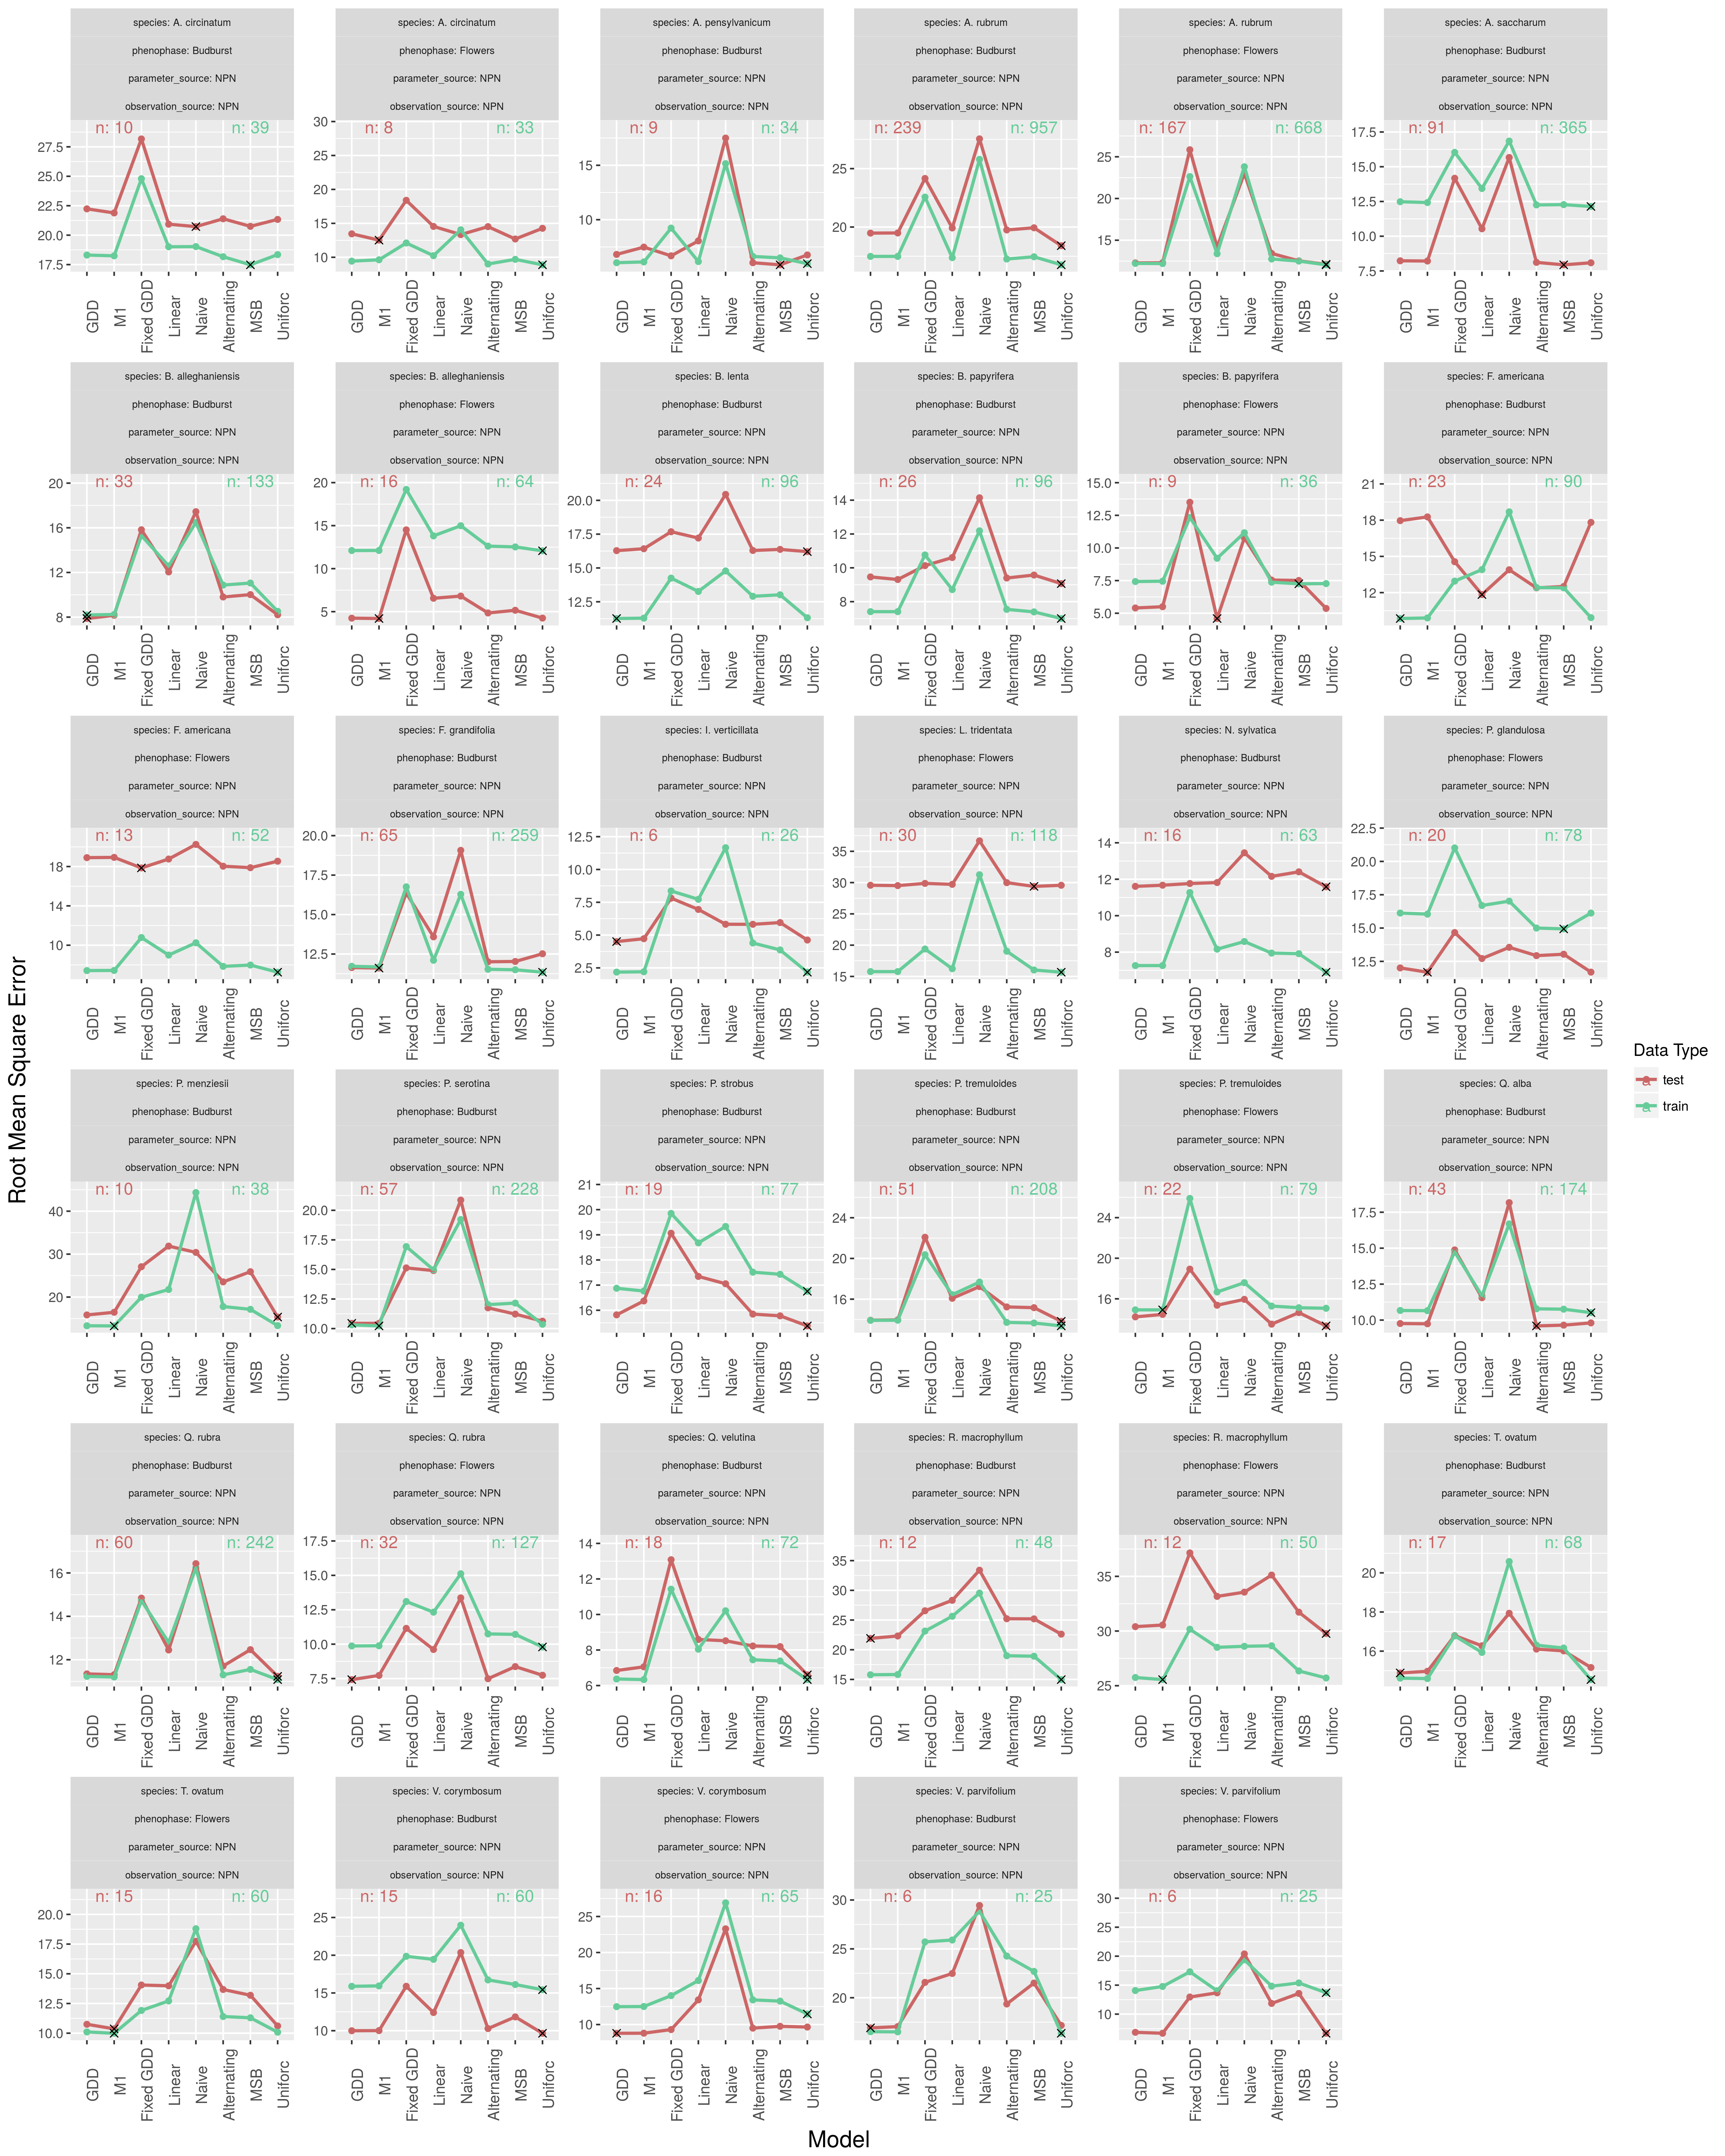
\includegraphics[width=1\textwidth]{supplement_best_npn_models.png}
\end{center}

\newpage
%%%%%%%%%%%%%%%%%
%% Figure S2
%%%%%%%%%%%%%%%%%
\textbf{Figure S2}: RMSE for specific species and phenophases of the LTER datasets. X marks the best performing models for the respective data type.

\newpage

\begin{center}
	\centering
		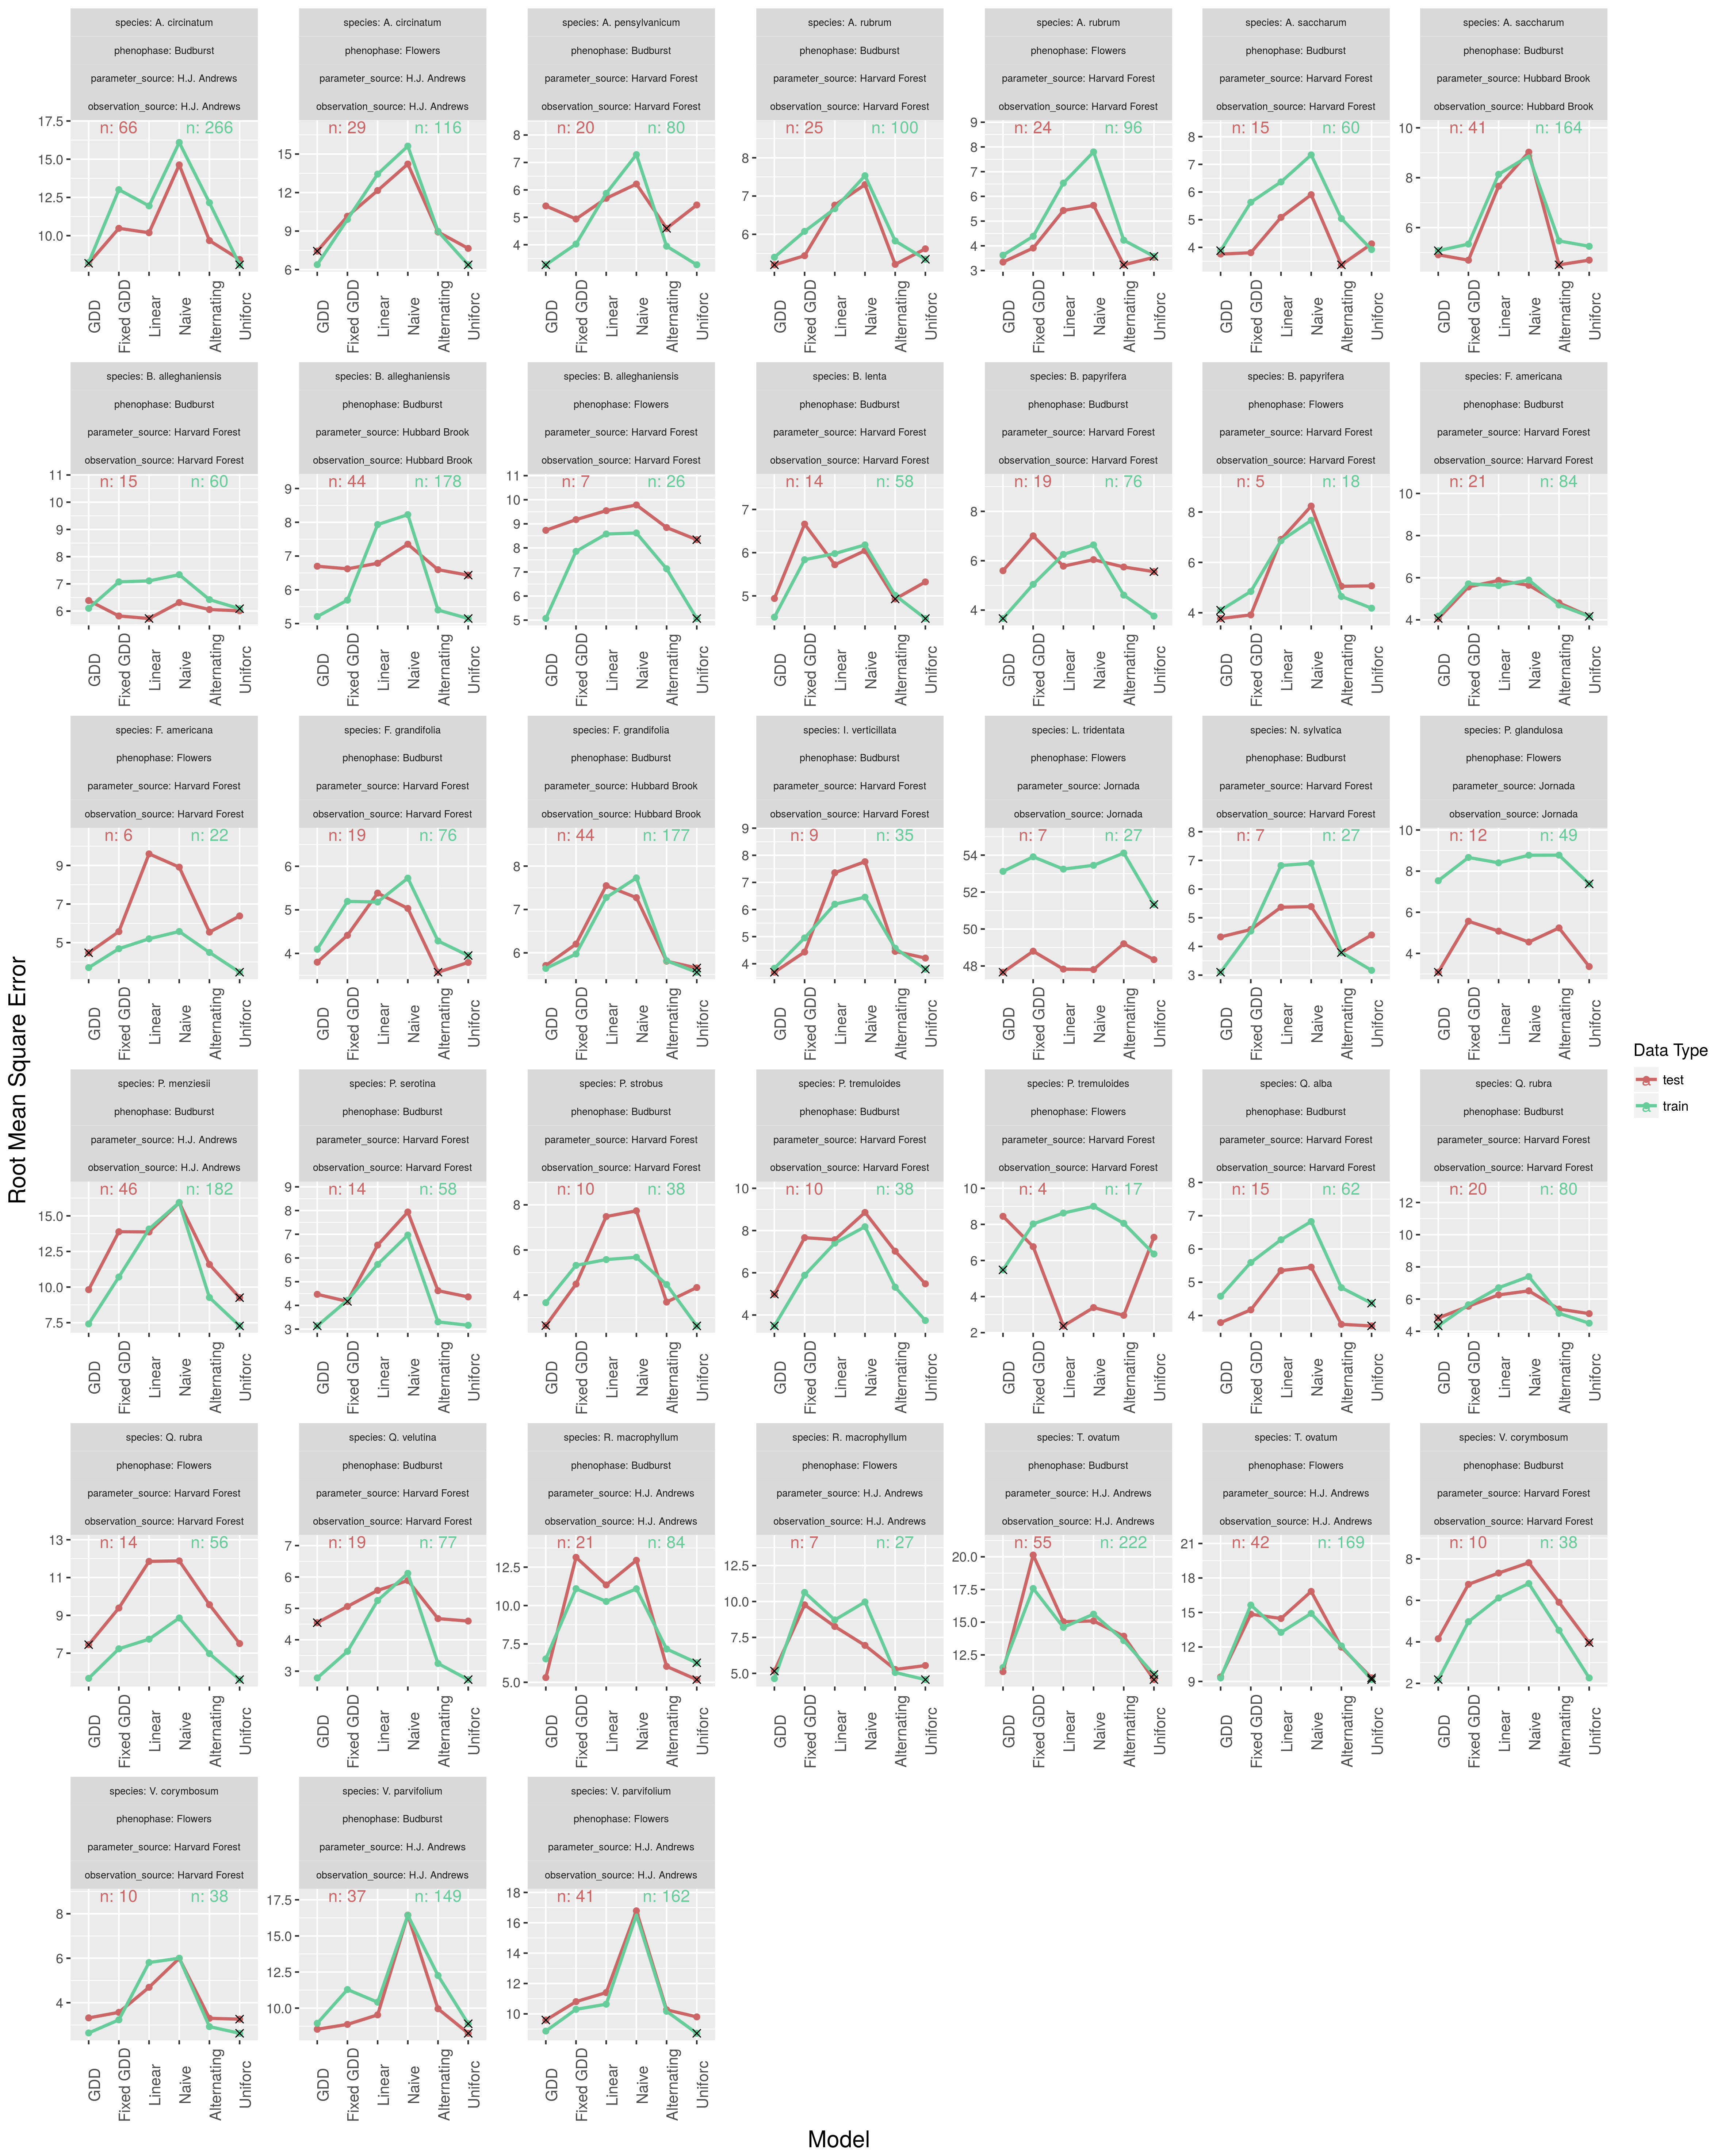
\includegraphics[width=1\textwidth]{supplement_best_lter_models.png}
	\caption{Figure S2}
\end{center}

%%%%%%%%%%%%%%%%%
%% Figure S3
%%%%%%%%%%%%%%%%%

\newpage

\textbf{Figure S3}: RMSE of all species and phenophases of the four scenarios described in the text. These values are calculated using held out test data.

\newpage

\begin{center}
	\centering
		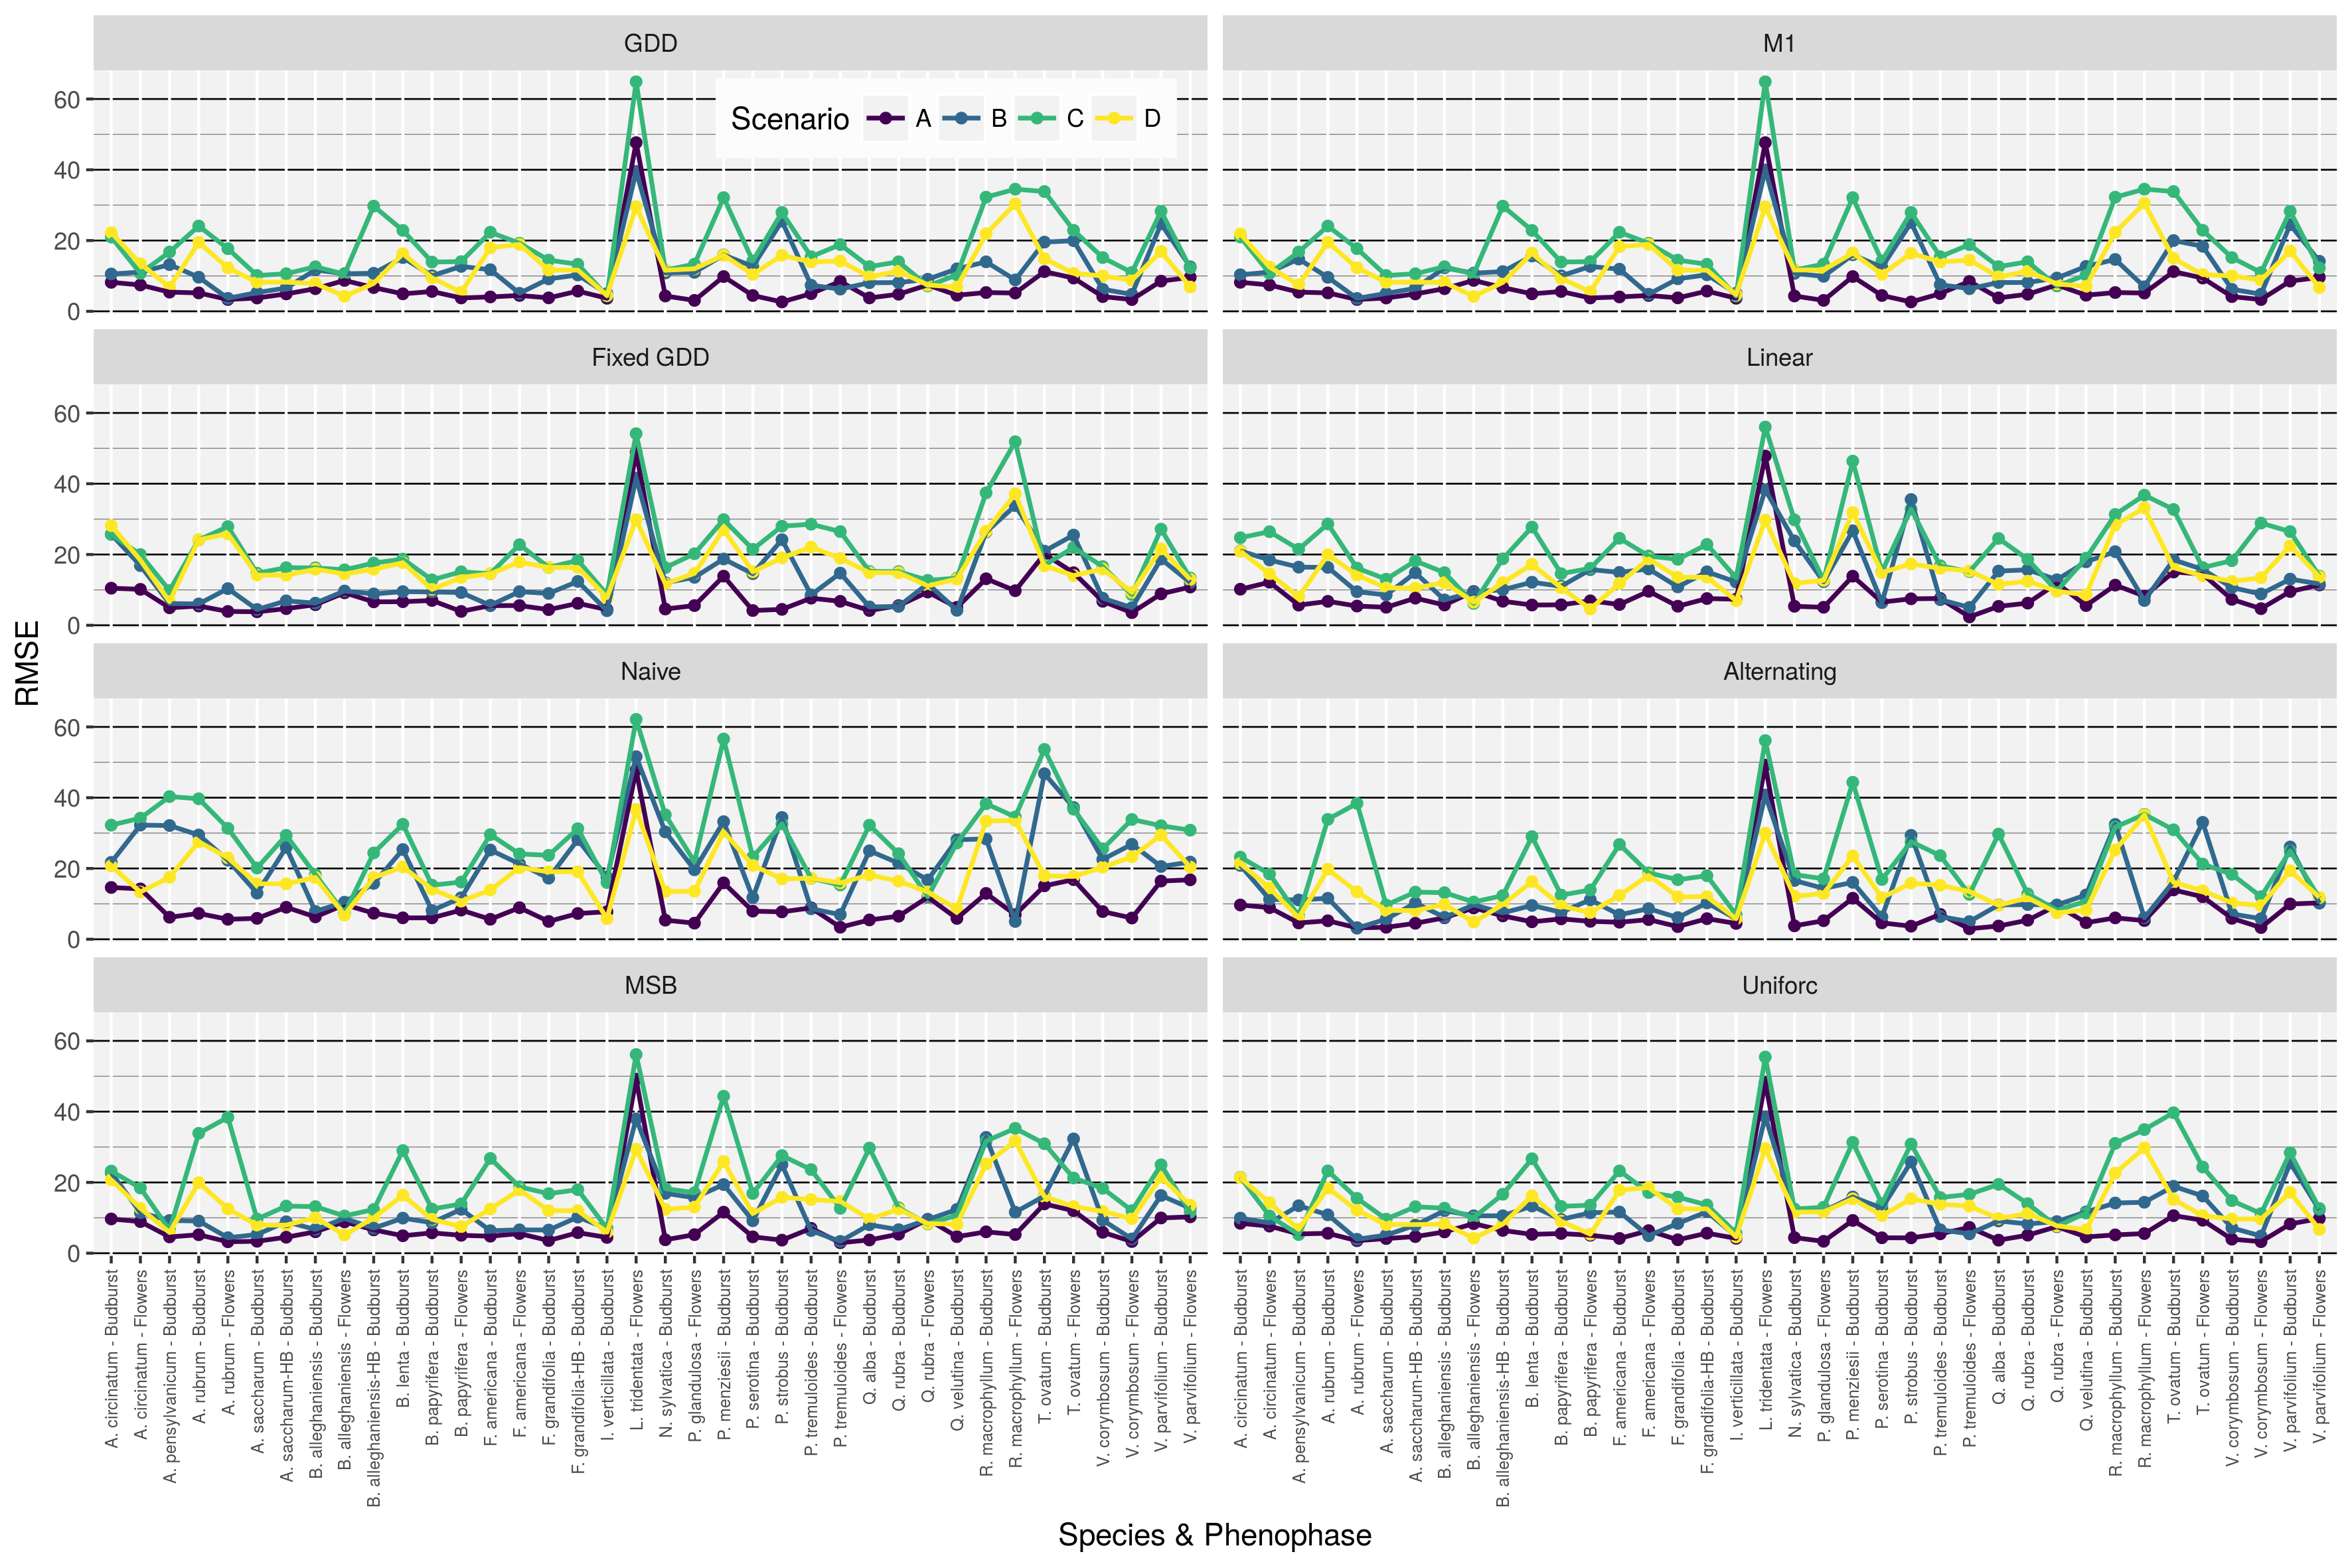
\includegraphics[width=1\textwidth]{supplement_scenario_absolute_rmse.png}
	\caption{Figure S3}
\end{center}

%%%%%%%%%%%%%%%%%
%% Figure S4
%%%%%%%%%%%%%%%%%
\newpage

\textbf{Figure S4}: Distribution of model parameters for the three species common to the Hubbard Brook, Harvard, and NPN datasets. The phenophase is budburst for all three species. Vertical lines indicate either the mean (solid) or median (dashed) of the respective distribution.

\newpage

\begin{center}
	\centering
		\includegraphics[width=1\textwidth]{supplement_hubbard_harvard_comparison.png}
	\caption{Figure S4}
\end{center}



\end{document}}
